\documentclass{article}
\usepackage[a4paper, total={6.5in, 8.5in}]{geometry}
\usepackage{graphicx}
\usepackage{booktabs}
\usepackage[label=corner]{karnaugh-map}
\usepackage{tabularray}
\usepackage{multicol}
\usepackage{multirow}
\usepackage{array}
\usepackage{hyperref}
\hypersetup{
    colorlinks=true,
    linkcolor=blue,
    }
\usepackage{float}
\usepackage{caption}
\usepackage{subcaption}
\usepackage[siunitx, RPvoltages]{circuitikz}
\usetikzlibrary{calc}
\usepackage{tikz, pgfplots}
\usetikzlibrary{positioning}
\usepackage{enumitem}
\usepackage{biblatex}
\usepackage{rotating}
\usepackage{ragged2e}




% Cover Page




\title{CSE 306 \\
Computer Architecture Sessional \\

\vspace{5mm}

\begin{figure}[h]
    \centering
    
\includegraphics[width=0.3\textwidth]{images/buet.png}
    \label{fig:enter-label}
\end{figure}

\vspace{5mm}
Assignment-1\\
4-bit ALU Simulation \\
\vspace{10mm}
Section - A1 \\
Group - 01 \\
\vspace{15mm}
\RaggedRight
Group Members: \\
\normalsize	{
\centering
\begin{enumerate}[]
    \item 2005001 - Anik Saha
    \item 2005012 - Abrar Jahin Sarker
    \item 2005013 - Al Muhit Muhtadi
    \item 2005017 - Abdullah Muhammed Amimul Ehsan
    \item 2005023 - Jaber Ahmed Deeder
\end{enumerate}
}
}
\author{}
\date{}




\begin{document}

\maketitle





% Section A-B - Anik





\section{Introduction}

First proposed by John Von Neumann, ALU stands as a cornerstone in the realm of computer architecture ever since its coinage in 1945. With diminishing transistor dimensions, implementing and incorporating wider-word ALUs in tiny microprocessors has kept becoming easier and cheaper. In the light of our own experimentation, this report aims at exploring the strategies of ALU design in considerable depth. We first provide a modest introduction to the theoretical foundation. Afterwards we present our methodology, outcomes and scopes of further exploration. 

\subsection{Definition}

An arithmetic logic unit abbreviated as ALU is a combinational digital circuit that performs arithmetic and bitwise operations on integer binary numbers.


\subsection{Overview}

Figure 1 presents a block diagram of a 4-bit ALU which takes two 4 bit numbers A($A_3A_2A_1A_0$) and B($B_3B_2B_1B_0$) as inputs and 3 control selection bits $cs_2, cs_1, cs_0$. After performing the operation, it outputs 5 bits namely, $C_{out}, S_3, S_2, S_1, S_0$ Additionally, it updates the 4 flags named S, C, V, Z in the Flags register accordingly.

\begin{figure}[htbp]
\centering
  \includegraphics[width=0.6\textwidth]{images/alu-block.png} 
  \caption{Block Diagram of 4 bit ALU}
  \label{fig:example}
\end{figure}

To generalize, the inputs for an  n-bit ALU are two n-bit binary numbers and k control selection bits, where the value of k is design specific. And it outputs an n-bit binary number S and one output carry. Alongside these, it calculates the 4-flags and store them in the Flags register.

\subsection{Components}

\subsubsection{Control Selection}

A number of mutually independent distinct input bits are used as control selection bits which determine the nature of the operation to be performed on the operands. Sometimes, one of these bits, usually the most significant one, is used solely to distinguish between arithmetic and logical operations. However, cases depending upon the requirements may well appear where one single bit is not adequate to meet this purpose. 


Each of the $2^{k}$ combinations of the possible inputs in the control bits is mapped to a single operation defined on the operands. It is, however, permissible to have multiple combinations of selection bits to map to the same operation. 

\subsubsection{Operands}

Two independent operands usually consisting of the same number of bits are fed into the ALU through circuitry. All operations determined by the control selection bits are applied on these two operands. 

For operations which do not impose symmetry upon the operands, for instance, subtraction, order of the operation matters. In this case, usually subtraction means subtraction of B from A. 

For bitwise logical operations, the corresponding action is performed bit by bit and the output is also generated bit by bit and no two distinct bits affect others’ outputs.

Operands are not usually used directly into the circuitry. Most often, each bit of an operand goes through identical circuitry and thus produces the corresponding input bits which need to be passed into the full adder.

\subsubsection{Arithmetic Unit}

Full adder, although usually interpreted as a circuitry for adding two n-bit numbers and generating the summation with output carry, can be utilized in multifaceted ways, thereby allowing a designer to efficiently perform seemingly disjoint arithmetic operations by intelligently manipulating the different input bits of a full adder. Regarding the full adder, one significant consideration is that, ideally the full-adder must include an internal carry-lookahead mechanism, Otherwise race conditions may appear and may pose to be an impediment towards accurate calculations.

Common arithmetic operations include transfer, addition, addition with carry, increment, decrement, subtraction, subtraction with borrow, negation (2’s complement). The mathematical interpretation of the aforementioned operations is presented in the table below:

\begin{center}
\begin{table}[h]
    \centering
\begin{tabular}{|c|c|}

\hline
\textbf{Name of operation} & \textbf{Equation}        \\ \hline
Transfer A              & A                  \\ \hline
Addition                & A + B              \\ \hline
Addition with Carry     & A + B + 1          \\ \hline
Subtraction             & A + B' + 1 (A - B) \\ \hline
Subtraction with borrow & A + B'  (A-B-1)    \\ \hline
Negation                & A' + 1 (-A)        \\ \hline

\end{tabular}
\caption{Arithmetic Operations}
\end{table}
\end{center}

\newpage
\subsubsection{Logic Unit}

Bitwise logical operations on n-bit operands is just as important in terms of computation as are the arithmetic ones. 
These operations include bitwise AND, OR, Exclusive-OR (XOR) and One's complement. But depending on requirements, more complex logical operations may as well be needed. The calculations of the logic unit may either be carried out in a separate circuit or may be incorporated into the arithmetic unit after careful manipulations. In the former case, additional circuit elements need to be introduced to merge the two units and to run the appropriate unit for respective selection of control bits.

Alongside bitwise logical operations, another type of bitwise operation named Logical Shift is often required. This may involve right shift, left shift or bit rotation. Whether this operation will be implemented inside a separate unit or inside the ones mentioned above is often a matter of design choice.

\subsubsection{Output}

Just as it happens in full adder, the output is generated as an n-bit number in the n distinct bits of the outputs of full adder. Additionally an extra bit named output carry ($C_{out}$) is generated. If overflow does not happen for the particular scenario, then the output corresponds to the result of the intended operation that is defined by the combination of the selection bits.

It is to note that, for some particular operations, the output is to be perceived after disregarding the output carry. For instance, since subtraction is carried out as 2’s complement, the output, when $C_{out}$ is considered, is actually equal to the desired result plus $2^n$. Therefore to interpret the correct difference between the operands, one needs to ignore the final output carry.

\subsubsection{Flags Register}

Last but not the least, an ALU leaves valuable information regarding the overall nature of the computation in a register called Flags Register. Usually there are 4 flags that are updated accordingly after performing the computations on the operands. However, in case of some operations, some particular flags may as well need to be kept constant.

The details regarding the equation and significance of each flag is shown in the table below:

\begin{center}
\begin{table}[h]
    \centering
\begin{tabular}{|l|c|p{10cm}|}

\hline
\textbf{Name of Flag} & \textbf{Equation} & \textbf{Significance}        \\ \hline

Sign (S)     & $S_3$       & It denotes the most significant bit of the output from full adder. Thus this flag helps determine  the sign of the output.                                                           \\ \hline
Carry (C)    & $C_{out}$   & It denotes the output carry.                                                                                                                                                         \\ \hline
Overflow (V) & $C_{out} \oplus C_{3}$ & This flag indicates whether there occurred an overflow while performing the calculation. If this flag is set, it means that the apparent output is not equal to the intended result and corrective measures must be taken while interpreting the output. \\ \hline
Zero (Z)     & $\overline{S_{3}+S_{2}+S_{1}+S_{0}}$         & It indicates whether all bits of the output are zero. \\ \hline

\end{tabular}
\caption{Equation and Significance of Flags}
\end{table}
\end{center}

\newpage
\subsection{Design Strategies}

With varying requirements, design strategies may differ from each other by a significant amount. Additionally, not all design processes focus on optimizing the same parameter. However, to broadly classify, the design process may incorporate one of the following two prevalent patterns:

\subsubsection{Disjoint Implementation}

One simple approach involves separate implementation of arithmetic and logic unit circuits. In this case, the Arithmetic unit is carried out with a full adder and the logic unit calculates the bitwise operations with direct involvement of corresponding gates and multiplexers. Then, to merge these two circuits, an additional multiplexer is needed to differentiate and determine which circuit will be active for which combinations.

While this approach seems easy to understand and implement, the major drawback is that, while combining the two circuits together, it needs a number of unnecessary ICs which may exceed size and cost restrictions.

\subsubsection{Unified Implementation}

An alternative approach considers converting the logical operations to equivalent arithmetic operations and thereby performing them in the same circuit as of the arithmetic one. Although the design process tends to get a bit complicated in this approach, the tradeoff is well worth it when the reduction in the number of ICs is considered.


\vspace{2cm}


\section{\large{Problem Specification with Assigned Instructions}}
Design a 4-bit ALU with three control selection bits $cs_0, cs_1, cs_2$. The assigned instructions and corresponding combinations of control selection bits are shown in the table below:
\begin{table}[h]
    \centering
    \begin{tabular}{||c|c|c|l|l||}
    \hline
         \multicolumn{3}{||c|}{Control Signals} & \multirow{2}{*}{Functions} & \multirow{2}{*}{Description}\\
         \cline{1-3}
         cs2 & cs1 & cs0 & & \\
         \hline
         \hline
         0 & X & 0 & Add & $A + B$ \\
         0 & 0 & 1 & Neg A & $-A(\overline{A}+1)$ \\
         0 & 1 & 1 & Add with Carry & $A + B + 1$\\
         1 & 0 & 0 & Increment A & $A + 1$\\
         1 & 0 & 1 & AND & $A . B$\\
         1 & 1 & X & XOR & $A \oplus B$\\
         \hline
    \end{tabular}
    \caption{Problem Specification}
    \label{tab:Table1}
\end{table}
\vspace{15mm}

\newpage







% Section C - Amim







\section{Detailed design steps with K-Maps}
\subsection{Design Steps}
\begin{enumerate}
  
    

    \item Here we have to perform four types of arithmetic operations (Add, Negation, Add with carry, Increment) and two types of logical operations(logical AND , logical XOR).

    \item For the adder,the first input $X_i$ is either $A_i$ or $\overline{A_i}$ or $A_i B_i$  or $A_i \oplus B_i$.We used a $4 \times 1$    multiplexer  for  each  bit.
     The MUX has  $S_{x_1}$ and $S_{x_0}$ as selection bits.The selection bits are controlled by control bits($c_{s_2}$,$c_{s_1}$,$c_{s_0}$).The details is shown in the truth table and k-Map.

     \item For the adder,the second input $Y_i$ is either $B_i$ or 0. We used a $2 \times 1$ multiplexer for each bit. 
     The mux has $S_{y_0}$ as its selection bit.The selection bit is controlled by control bits($c_{s_2}$,$c_{s_1}$,$c_{s_0}$).The details in shown in the truth table and k-Map.

    \item The input carry($C_{in}$) of the adder IC is either 0 or 1.It should be zero for negation, add with carry, and increment operations.This is also controlled by control bits($c_{s_2}$,$c_{s_1}$,$c_{s_0}$).The details is shown in the truth table and k-Map.

    \item In the arithmetic unit, the adder adds $A$, $B$ with $C_{in}=0$ and $C_{in}=1$ for Add, Add with Carry operations respectively. The multiplexers provide $Y_i$ as a 0 for increment operation.During negation,$X_i$=$\overline{A_i}$ and $Y_i$=0 and $C_{in}$=1. 
    
    \item During logical operations,$X_i$ is transferred as $Y_i$=0 and $C_{in}$=0.

    \item Zero flag, ZF is computed by adding the 4 output bits using 3 OR gates and then inverting $O_0 + O_1+O_2+O_3$ by 1 XOR gate($X\oplus1=\overline{X}$).
    \item The carry flag($C$) is directly obtained from $C_{out}$ of the parallel adder
    \item The sign flag(SF) is obtained from the MSB of the sum($S_3$).
    \item  For the overflow flag,we needed $C_{out}$ and $C_3$. $C_{out}$ is directly accessible from the Adder IC. $C_3$ is calculated as below:
    \begin{center}
        $S_3$ = $X_3 \oplus Y_3 \oplus C_3$\\
        $S_3 \oplus C_3$ = $X_3 \oplus Y_3$\\
        $C_3$ = $X_3 \oplus Y_3 \oplus S_3$\\
        OF = $C_{out} \oplus C_3$\\
        OF = $C_{out} \oplus X_3 \oplus Y_3 \oplus  S_3$
        
        
    \end{center}
        

\end{enumerate}

\subsection{K-maps}
We will be following Table 5 and 6 to construct the K-maps for selection bits of multiplexers and $C_{in}$.\\

% \subsubsection{K-maps for $S_{x_1}$ and $S_{x_0}$}
The IC of parallel adder takes $X_i$ and $Y_i$ and $C_{in}$ as input.We need  $X_i$  as $A_i$ or its complement or its logical changes with B.This values are  received as $X_i$(output of the multiplexer) and the kmap for selection bits($S_{x_1}$ and $S_{x_0}$) of the multiplexer are as follows:\\


\subsubsection{K-map for $S_{x_1}$}
\begin{center}
\begin{karnaugh-map}[2][4][1][$cs0$][$cs1$][$cs2$]
    \minterms{5,6,7}
    \maxterms{0,1,2,3,4}
    \implicant{7}{5}
    \implicant{6}{7}
\end{karnaugh-map}
\end{center}
We can easily express $S_{x_1}$ as sum of minterms. 

\[S_{x_1}=c_{s_2}c_{s_1}+ c_{s_2}c_{s_0}\]
\[S_{x_1}=c_{s_2}(c_{s_1}+c_{s_0})\]




\subsubsection{K-map for $S_{x_0}$}

\begin{center}
\begin{karnaugh-map}[2][4][1][$cs0$][$cs1$][$cs2$]
    \minterms{1,5}
    \maxterms{0,2,3,4,6,7}
    \implicantedge{1}{1}{5}{5}
    %\implicant{6}{7}
\end{karnaugh-map}
\end{center}
So, there are two minterms.
\[ S_{x_0} = {\overline{c_{s_1}}c_{s_0}}\]



\subsubsection{K-map for $S_{y_0}$}
$S_{y_0}$ is the selection bit for the multiplexer that selects B and 0 as input of a 2*1 MUX .
\begin{center}
\begin{karnaugh-map}[2][4][1][$cs0$][$cs1$][$cs2$]
    \minterms{1,4,5,6,7}
    \maxterms{0,2,3}
    \implicantedge{1}{1}{5}{5}
    \implicant{6}{5}
\end{karnaugh-map}
\end{center}


\[ S_{y_0} =  = {c_{s_2}+\overline{c_{s_1}}c_{s_0}}\]

\subsubsection{K-map for $C_{in}$}
It is the input carry bit of the adder used inside arithmetic unit.
\begin{center}
\begin{karnaugh-map}[2][4][1][$cs0$][$cs1$][$cs2$]
    \minterms{1,3,4}
    \maxterms{0, 2,  5,6,7}
    \implicant{1}{3}
    \implicant{4}{4}
\end{karnaugh-map}
\end{center}
\[C_{in}=\overline{c_{s_2}}c_{s_0}+c_{s_2}\overline{c_{s_1}}.\overline{c_{s_0}}\]
\[C_{in}=\overline{c_{s_2}}c_{s_0}+c_{s_2}.\overline{c_{s_1}+c_{s_0}}\]







% Section D - Muhit



\section{\large{Truth Table}}

\begin{table}[H]
	\centering
	\begin{tabular}{|c|c|c|c|c|c|c|c|c|}
		\hline
		cs2 & cs1 & cs0 & $X_{i}$ & $Y_i$ & $Z_{i}$ & $C_{in}$ & Function  \\
		\hline
		0 & 0 & 0 & $A_{i}$ & $B_{i}$ & $C_{i}$ & 0 & Add \\
		0 & 0 & 1 & $\overline{A_i}$ & 0 & $C_i$ & 1 & NEG A \\
		0 & 1 & 0 & $A_{i}$ & $B_{i}$ & $C_{i}$ & 0 & Add \\
		0 & 1 & 1 & $A_{i}$ & $B_{i}$ & $C_{i}$ & 1 & Add with carry \\
		1 & 0 & 0 & $A_i$ & 0 & $C_i$ & 1 & Increment A \\
		1 & 0 & 1 & $A_{i}B_{i}$ & 0 & $C_i$ & 0 & AND \\
		1 & 1 & 0 & $A_i \oplus B_i$ & 0 & $C_i$ & 0 & XOR \\
		1 & 1 & 1 & $A_i \oplus B_i$ & 0 & $C_i$ & 0 & XOR \\
		\hline
	\end{tabular}
	\caption{Truth Table of $X_i$, $Y_i$, $Z_i$, $C_{in}$}
	\label{tab:truth_table1}
\end{table}
\begin{table}[H]
	\centering
	\begin{tabular}{|c|c|c|c|c|c|}
		\hline
		cs2 & cs1 & cs0 & $X_{i}$ & $S_{x_1}$ & $S_{x_0}$  \\
		\hline
		0 & 0 & 0 & $A_{i}$ & 0 & 0 \\
		0 & 0 & 1 & $\bar{A_i}$ & 0 & 1 \\
		0 & 1 & 0 & $A_{i}$ & 0 & 0 \\
		0 & 1 & 1 & $A_{i}$ & 0 & 0 \\
		1 & 0 & 0 & $A_i$ & 0 & 0\\
		1 & 0 & 1 & $A_{i}B_{i}$ & 1 & 1\\
		1 & 1 & 0 & $A_i \oplus B_i$ & 1 & 0 \\
		1 & 1 & 1 & $A_i \oplus B_i$ & 1 & 0 \\
		\hline
	\end{tabular}
	\caption{Truth Table of MUX input for $X_i$}
	\label{tab:truth_table2}
\end{table}

\begin{table}[H]
	
	\centering
	\begin{tabular}{|c|c|c|c|c|}
		\hline
		cs2 & cs1 & cs0 & $X_{i}$ & $S_{y_0}$  \\
		\hline
		0 & 0 & 0 & $B_{i}$ & 0 \\
		0 & 0 & 1 & 0 & 1 \\
		0 & 1 & 0 & $B_{i}$ & 0  \\
		0 & 1 & 1 & $B_{i}$ & 0  \\
		1 & 0 & 0 & 0 & 1\\
		1 & 0 & 1 & 0 & 1\\
		1 & 1 & 0 & 0 & 1\\
		1 & 1 & 1 & 0 & 1\\
		\hline
	\end{tabular}
	\caption{Truth Table of MUX input for $Y_i$}
	\label{tab:truth_table3}
\end{table}







% Section E-F - Jahin





\section{\large{Block Diagram}}
\vspace{15mm}
\begin{figure}[H]
    \centering
    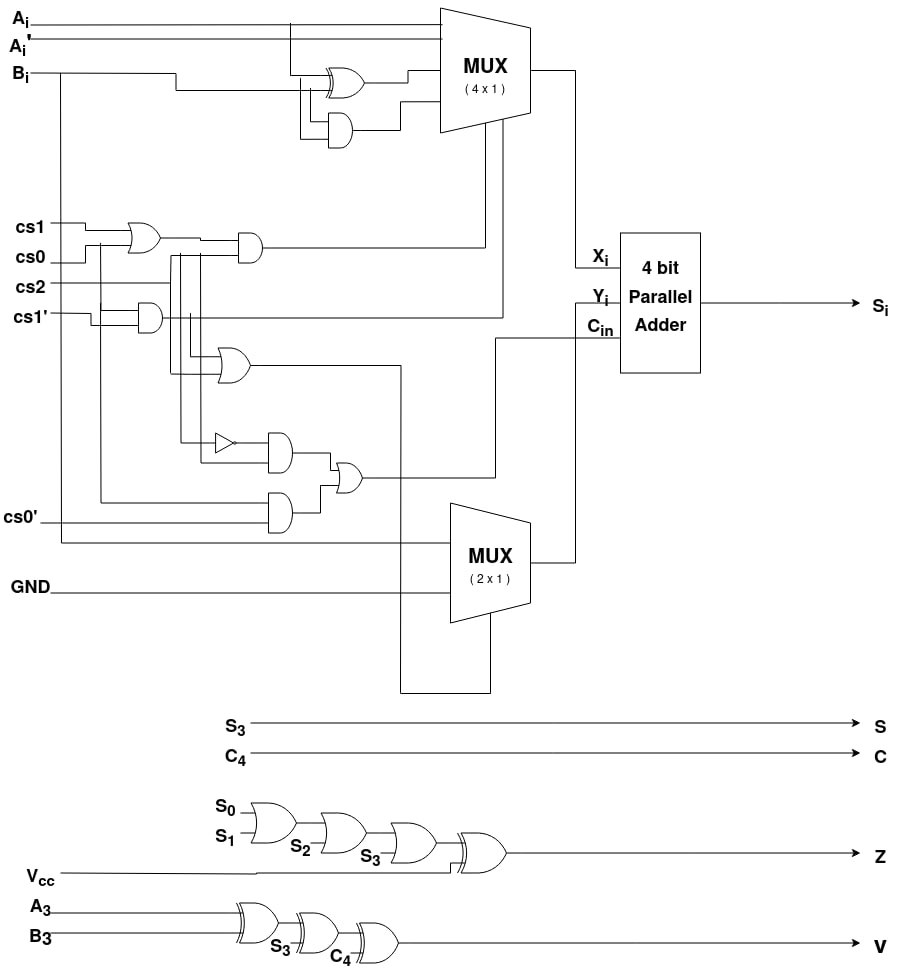
\includegraphics[width=0.8\textwidth]{images/block-new.jpg}
    \caption{ Block Digram of ALU }
    \label{fig:enter-label}
\end{figure}
% \ctikzset{
%     logic ports=ieee,
%     logic ports/scale=1
% }

\section{\large{Complete Circuit Diagram}}

     \begin{figure}[H]
         \centering
         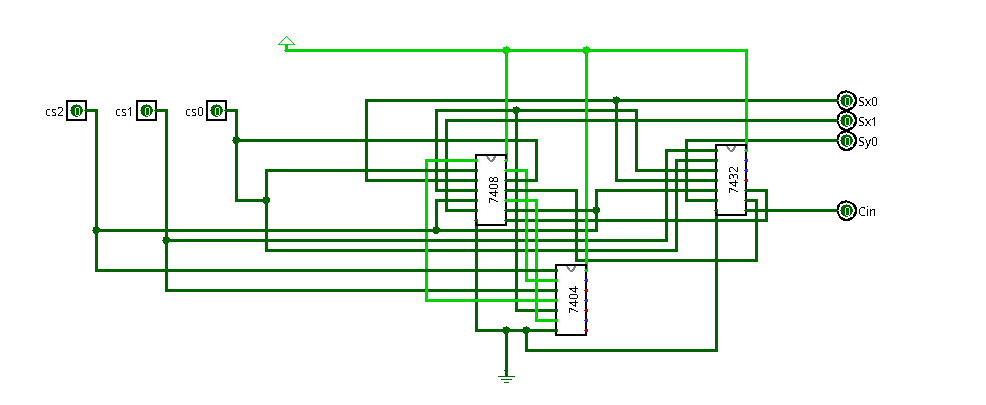
\includegraphics[width=0.8\textwidth]{images/control_preprocessor.png}
         \caption{Control Processing Unit}
         \label{fig:alu_a}
     \end{figure}
     \begin{figure}[H]
         \centering
         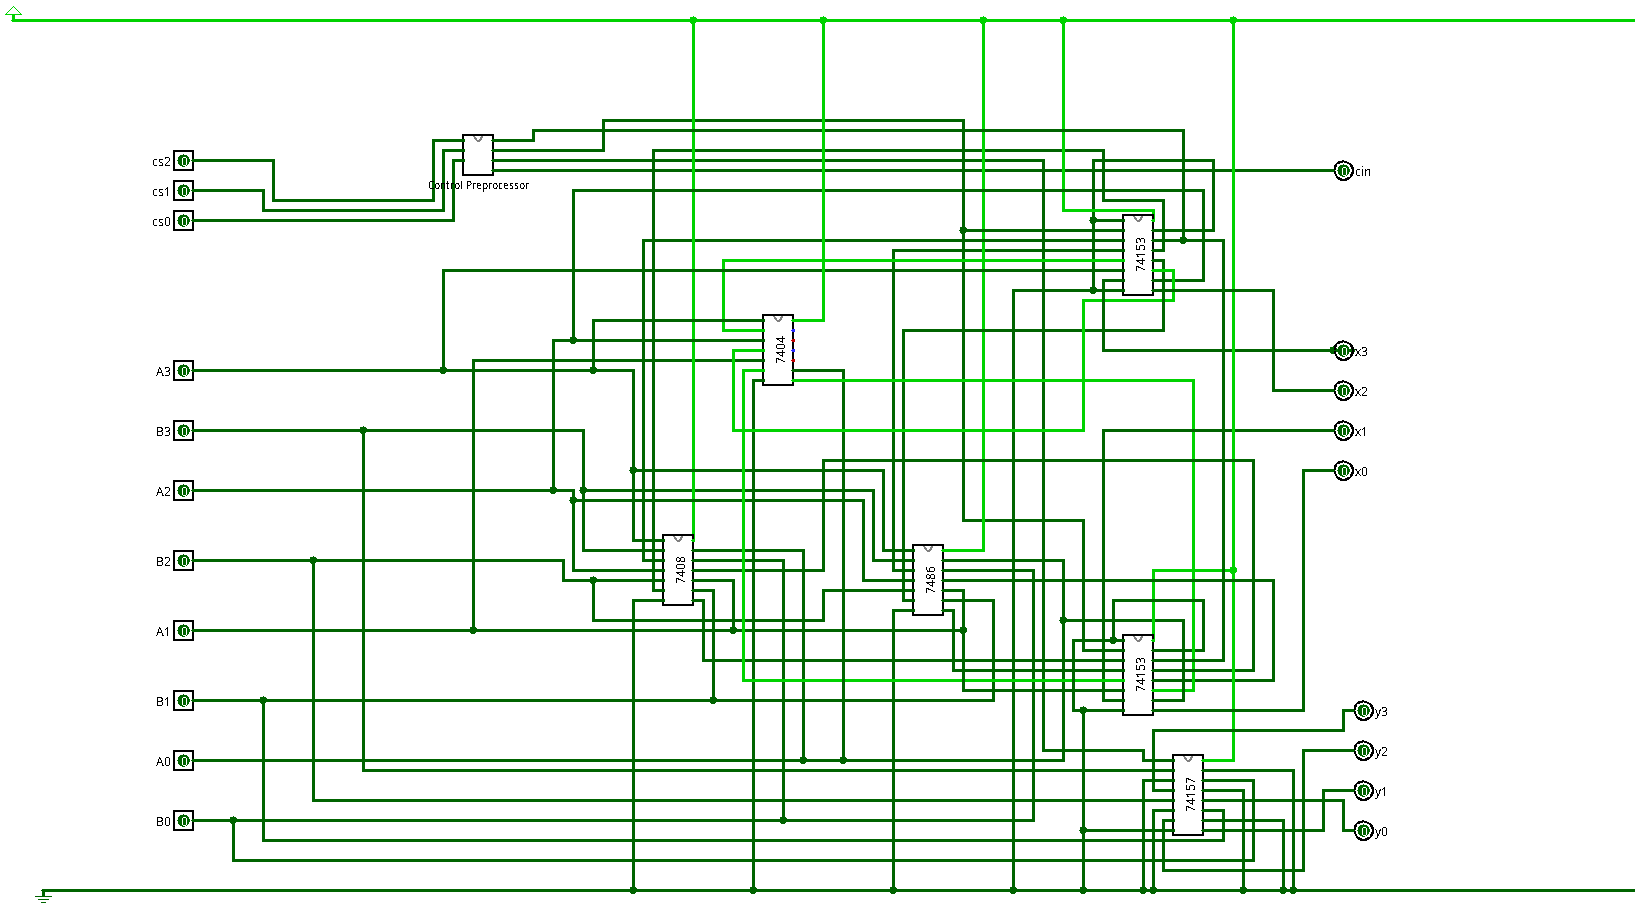
\includegraphics[width=0.8\textwidth]{images/input_preprocessor.png}
         \caption{Input Processing Unit}
         \label{fig:alu_b}
     \end{figure}
     \begin{figure}[H]
         \centering
         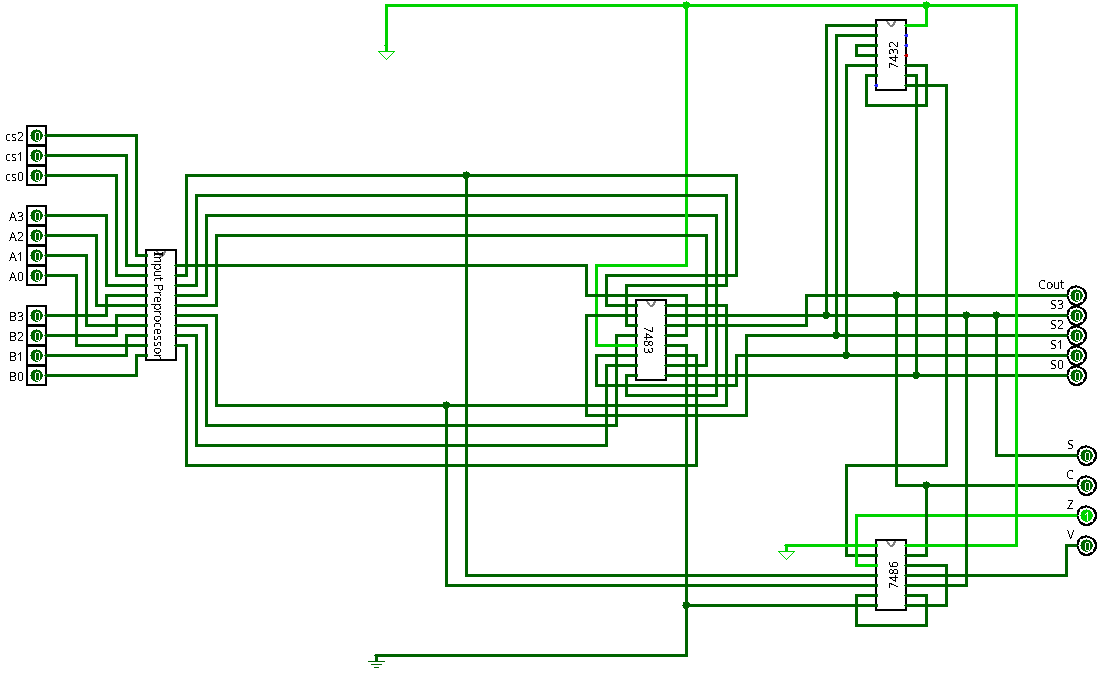
\includegraphics[width=0.8\textwidth]{images/main.png}
         \caption{Arithmetic Logic Unit (ALU)}
         \label{fig:alu_c}
     \end{figure}



\newpage


% Section G - Jaber


	
\section{\large{ICs Used with Count as a Chart}}

\begin{table}[!h]
	\centering
	\begin{tabular}{|c|c|}
		\hline
		\textbf{IC} & \textbf{Quantity}  \\
		\hline
		IC 74153 & 2 \\
		IC 74157 & 1 \\
		IC 7408 & 2 \\
		IC 7432 & 2 \\
		IC 7404 & 2 \\
		IC 7486 & 2 \\
		IC 7483 & 1 \\
		\hline
		Total & 12  \\
		\hline
	\end{tabular}
	\caption{ICs Used with Quantity}
	\label{tab:ic_quantity}
\end{table}





% Section H-J - Combined




\vspace{5mm}
\section{The Simulator Used along with the Version Number}
Logisim - 2.7.1
 \newpage

\section{Discussion}


The assignment on the implementation of ALU, our very first step onto the intricate realm of hardware design, assisted in strengthening and solidifying our understanding of the internal building block of computing in multifaceted dimensions. Alongside serving as a practical visualizer for our theoretical knowledge, the task helped refurbish our problem solving strategies and optimization techniques to a considerable extent.

\vspace{2mm}

The design was meticulously crafted with a primary focus on optimization, prompting subsequent refinement to minimize the count of integrated circuits (ICs). Our requirement for input variables X and Y, encompassing A, A' (complement of A), AB, A XOR B for X, and B, B' for Y, necessitated a thoughtful approach. While the multiplexer provided the expected X and Y, our commitment to utilizing basic gates and XOR gates compelled us to generate inputs for the MUX systematically. 

\vspace{2mm}

In the input preprocessor, intermediate adder inputs were calculated and produced efficiently. MUX's were used to reduce IC counts. The attached truth tables depict relationships with various inputs with control bits. Expressions for flags were calculated with maximum accuracy.

\vspace{2mm}

4 position DIP switches were used to give inputs to the circuit. Their main advantages are that they are quicker to change and provide a visual indication of the position of the switch, making it easier for the user to understand the functioning of the circuit.

\vspace{2mm}

Rigorous testing and step-by-step debugging were integral to our circuit implementation process. During debugging, meticulous attention was devoted to ensuring all essential connections. Any potential incorrect connections were rectified. Additionally, vigilant checks were conducted to prevent inadvertent shorts in wires or components. Verifying the actual polarity of LEDs and other instruments was paramount. To enhance the debugging process, an extra LED was strategically connected, enabling us to validate the correctness and expected output at every stage of development.

\vspace{2mm}

Backtracking was necessary to debug several mis-produced outputs. Care was taken so that no two wires become short circuited. Ground and Vcc pins of IC's were connected correctly.

\vspace{2mm}

To obtain simplified expressions and to compare the corresponding IC counts over a bulk set of choices, a python script was used. The script scraped the output from a website and delivered that to another pipeline, thereby automating the process. Wires and resistors were reduced to small sizes using wire strippers to make the circuit cleaner. Black tape and double sided tapes were used to provide structural integrity. For extensive verification and testing, a python script was used to randomly generate test cases and their corresponding solutions to check if the circuit is working correctly.

\vspace{2mm}

To recapitulate, we exerted our fullest efforts onto a correct and optimized implementation. We are grateful to our supervisor, teachers and peers for their priceless assistance. We hope to explore this core concept of Computer Architecture in greater depth in future.



 
\newpage

\section{Contribution of Each Member}



\subsection{Logic Design and Simplification of Expressions}



\begin{table}[h]
    \centering
\begin{tabular}{|c|c|m{10cm}|}
\hline
Student ID & Surname & Contribution \\ \hline
2005001    & Anik    & Prepared block diagram with IC pin numbers mentioned, obtained simplified expressions for $Sx_1$, $Sx_0$, $Sy_0$             \\ \hline
2005012    & Jahin   &  Prepared truth tables for $Sx_1$, $Sx_0$, $Sy_0$             \\ \hline
2005013    & Muhit   &  Prepared truth tables for $X_i$, $Y_i$, $C_{in}$            \\ \hline
2005017    & Amim    &  Prepared block diagram with IC pin numbers mentioned, obtained simplified expressions for  $X_i$, $Y_i$, $C_{in}$      \\ \hline
2005023    & Jaber   &  Obtained primary expressions for the Flags $Z$(Zero Flag) and $V$(Overflow Flag)     \\ \hline
\end{tabular}
\end{table}



\subsection{IC Count Optimization}



\begin{table}[h]
    \centering
\begin{tabular}{|c|c|m{10cm}|}
\hline
Student ID & Surname & Contribution \\ \hline
2005001    & Anik    & Performed optimal manipulations in preprocessing to reduce the number of IC $7408$, replaced a NOT gate with XOR gate to lessen one extra IC $7404$            \\ \hline
2005012    & Jahin   &  Developed synchronization among distinct modules to efficiently use maximum ports of ICs and to keep the modules disjoint            \\ \hline
2005013    & Muhit   &  Introduced the possibility of using MUX to avoid using too many gates in preprocessing, resolved errors related to optimization           \\ \hline
2005017    & Amim    &  Found a way of determining Overflow without explicitly obtaining the penultimate carry, thereby reducing one extra IC $7483$, finalized the solution containing 12 ICs      \\ \hline
2005023    & Jaber   &  Wrote a Python bot to scrape SOP forms from the website \href{http://www.32x8.com/index.html}{32x8.com} for automated comparisons            \\ \hline
\end{tabular}
\end{table}



\subsection{Logisim Simulation}


\begin{table}[h]
    \centering
\begin{tabular}{|c|c|p{10cm}|}
\hline
Student ID & Surname & Contribution \\ \hline
2005001    & Anik    & Developed Control Preprocessor which generates $Sx_1$, $Sx_0$, $Sy_0$, $C_{in}$ from $cs_2$, $cs_1$, $cs_0$            \\ \hline
2005012    & Jahin   & Developed the circuitry of the full adder (IC $7483$)  which generates $S_3$, $S_2$, $S_1$, $S_0$          \\ \hline
2005013    & Muhit   &  Developed Input preprocessor (jointly) which generates $X_i$, $Y_i$ from $A_i$, $B_i$, $Sx_1$, $Sx_0$, $Sy_0$      \\ \hline
2005017    & Amim    &  Developed Input preprocessor (jointly) which generates $X_i$, $Y_i$ from $A_i$, $B_i$, $Sx_1$, $Sx_0$, $Sy_0$      \\ \hline
2005023    & Jaber   &  Developed the circuitry of flags calculation which generates $S$, $C$, $Z$, $V$     \\ \hline
\end{tabular}
\end{table}

\newpage

\subsection{Hardware Implementation}



\begin{table}[h]
    \centering
\begin{tabular}{|c|c|p{10cm}|}
\hline
Student ID & Surname & Contribution \\ \hline
2005001    & Anik    & Developed Control Preprocessor which generates $Sx_1$, $Sx_0$, $Sy_0$, $C_{in}$ from $cs_2$, $cs_1$, $cs_0$, assisted in developing the circuitry of Full Adder and flags calculation            \\ \hline
2005012    & Jahin   & Developed a switching circuit for controlling the 11 input bits through three 4-bit DIP switches, also assisted in developing an output viewer circuit consisting of LEDs    \\ \hline
2005013    & Muhit   &  Developed Input preprocessor (jointly) which generates $X_i$, $Y_i$ from $A_i$, $B_i$, $Sx_1$, $Sx_0$, $Sy_0$ and assisted in the circuitry of Full Adder and flags calculation   \\ \hline
2005017    & Amim    &  Developed Input preprocessor (jointly) which generates $X_i$, $Y_i$ from $A_i$, $B_i$, $Sx_1$, $Sx_0$, $Sy_0$ and assisted in the circuitry of Full Adder and flags calculation    \\ \hline
2005023    & Jaber   &  Assisted in developing an output viewer circuit consisting of LEDs, finalized the hardware with improvements in structural integrity     \\ \hline
\end{tabular}
\end{table}



\subsection{Verification and Testing}



\begin{table}[h]
    \centering
\begin{tabular}{|c|c|p{10cm}|}
\hline
Student ID & Surname & Contribution \\ \hline
2005001    & Anik    & Developed a python script for verifying the generated truth table in Logisim through comparison with given functions           \\ \hline
2005012    & Jahin   & Refurnihsed the switching circuit for easy inputting mechanism, Performed random testing    \\ \hline
2005013    & Muhit   &  Performed extensive random testing and resolved bugs through backtracking   \\ \hline
2005017    & Amim    &  Performed crucial debugging while performing the verification process, performed random testing   \\ \hline
2005023    & Jaber   &  Developed a python script for randomly generating testcases and their corresponding solutions based on given control bits    \\ \hline
\end{tabular}
\end{table}



\subsection{Report Preparation}



\begin{table}[h]
    \centering
\begin{tabular}{|c|c|p{10cm}|}
\hline
Student ID & Surname & Contribution \\ \hline
2005001    & Anik    & Section $A$, $B$, $J$           \\ \hline
2005012    & Jahin   & Section $E$, $F$    \\ \hline
2005013    & Muhit   & Section $D$   \\ \hline
2005017    & Amim    & Section $C$  \\ \hline
2005023    & Jaber   & Section $G$, $H$    \\ \hline
\end{tabular}
\end{table} 


\end{document}

